\documentclass{standalone}
\usepackage{tikz, xcolor}
\usetikzlibrary{shapes,arrows}

\begin{document}

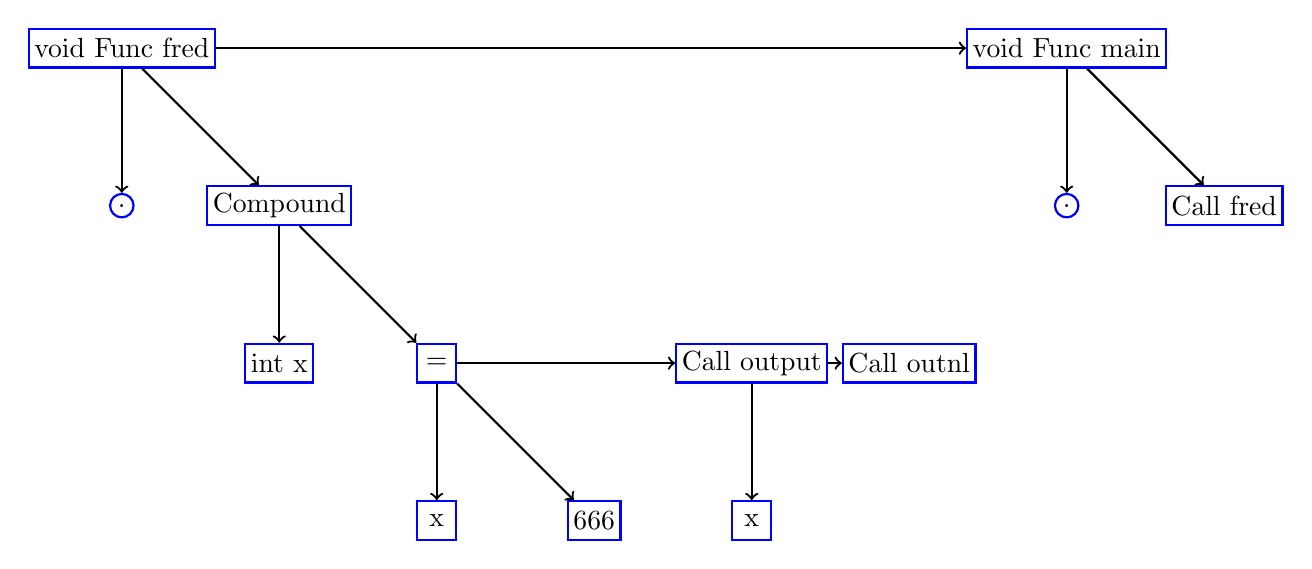
\begin{tikzpicture}[thick, scale=2.0]
\tikzstyle{vertexr}=[rectangle, draw=blue, thick, minimum size=14pt, inner sep=2pt]
\tikzstyle{vertexc}=[circle, draw=blue, thick, inner sep=2pt]
\tikzstyle{drawstyle}=[thick, ->]

\node[vertexr] (G0x0) at (0,0) {void Func fred};
\node[vertexc] (G0x1) at (0,-1) {.};
\draw[drawstyle] (G0x0) -- (G0x1);
\node[vertexr] (G1x1) at (1,-1) {Compound};
\node[vertexr] (G1x2) at (1,-2) {int x};
\draw[drawstyle] (G1x1) -- (G1x2);
\node[vertexr] (G2x2) at (2,-2) {=};
\node[vertexr] (G2x3) at (2,-3) {x};
\draw[drawstyle] (G2x2) -- (G2x3);
\node[vertexr] (G3x3) at (3,-3) {666};
\draw[drawstyle] (G2x2) -- (G3x3);
\node[vertexr] (G4x2) at (4,-2) {Call output};
\node[vertexr] (G4x3) at (4,-3) {x};
\draw[drawstyle] (G4x2) -- (G4x3);
\node[vertexr] (G5x2) at (5,-2) {Call outnl};
\draw[drawstyle] (G4x2) -- (G5x2);
\draw[drawstyle] (G2x2) -- (G4x2);
\draw[drawstyle] (G1x1) -- (G2x2);
\draw[drawstyle] (G0x0) -- (G1x1);
\node[vertexr] (G6x0) at (6,0) {void Func main};
\node[vertexc] (G6x1) at (6,-1) {.};
\draw[drawstyle] (G6x0) -- (G6x1);
\node[vertexr] (G7x1) at (7,-1) {Call fred};
\draw[drawstyle] (G6x0) -- (G7x1);
\draw[drawstyle] (G0x0) -- (G6x0);
\end{tikzpicture}
\end{document}
Number of warnings: 0
Number of errors: 0
